\documentclass[type = bachelor]{whu-thesis}
\usepackage{textcomp,mathcomp}
\usepackage{siunitx}
\usepackage{chemfig}
\usepackage{graphicx}

\whusetup
  {
    info               =
      {
        title          = {金刚石氮-空位色心的\\电荷态调控和性质表征},
        title*         = {Modulation of Charge States and Characterization of Properties\\ in Nitrogen-Vacancy Centers of Diamond},
        student-number = {2020302192129},
        school         = {弘毅学堂},
        author         = {邹迪玮},
        author*        = {Diwei Zou},
        subject        = {学科},
        major          = {微电子科学与工程},
        advisor        = {周利 , 副教授;孙启超 , 研究员},
        direction      = {研究方向},
        date           = {2024/5},
        keywords       = {关键词 1 , 关键词 2 , 关键词 3 , 关键词 4 , 一个非常非常,非常非常长——的关键词 5},
        keywords*      = {key word 1 , key word 2 , key word 3 , key word 4 , {and a very very, very very long key word---the key word 5}},
      },
    style              =
      {
        graphics-path  = {{figures/}{data/}},
        list-of-figures,
        list-of-tables,
      },
    element            =
      {
        innovation     = {pages/innovation},
        abstract       = {pages/abstract},
        abstract*      = {pages/enabstract},
        bibliography   = {ref/refs_2}
      }
  }
\begin{document}


% Chapter 2

\chapter{NV Center电荷态动力学的理论原理}

\section{NV Center的电荷态}
因为NV Center电荷态的一些最基本的性质和特征已经在第一章中有所分析,所以本章主要聚焦于NV Center电荷态动力学的理论原理,也就是本文后续实验中所主要研究的对象和内容。本文主要研究的对象是NV Center的负电状态NV$^-$和中性状态NV$^0$,而NV Center的正电状态NV$^+$由于其电子结构的特殊性,其电荷态动力学的研究相对较少,所以本文不做过多的讨论\cite{schreyvogel2016active}。

\subsection{NV Center电荷态的荧光光谱}

在第一章的图 1.7中,我们可以看到NV Center的不同电荷态的荧光发射光谱的特征。在NV Center的荧光光谱中,我们可以看到NV$^-$和NV$^0$的荧光峰分别位于$637$ nm和$575$ nm处,。在实验中,我们可以通过测量NV Center的荧光光谱来判断其电荷态,从而可以对NV Center的电荷态进行观测和表征。

\begin{figure}
  \centering
  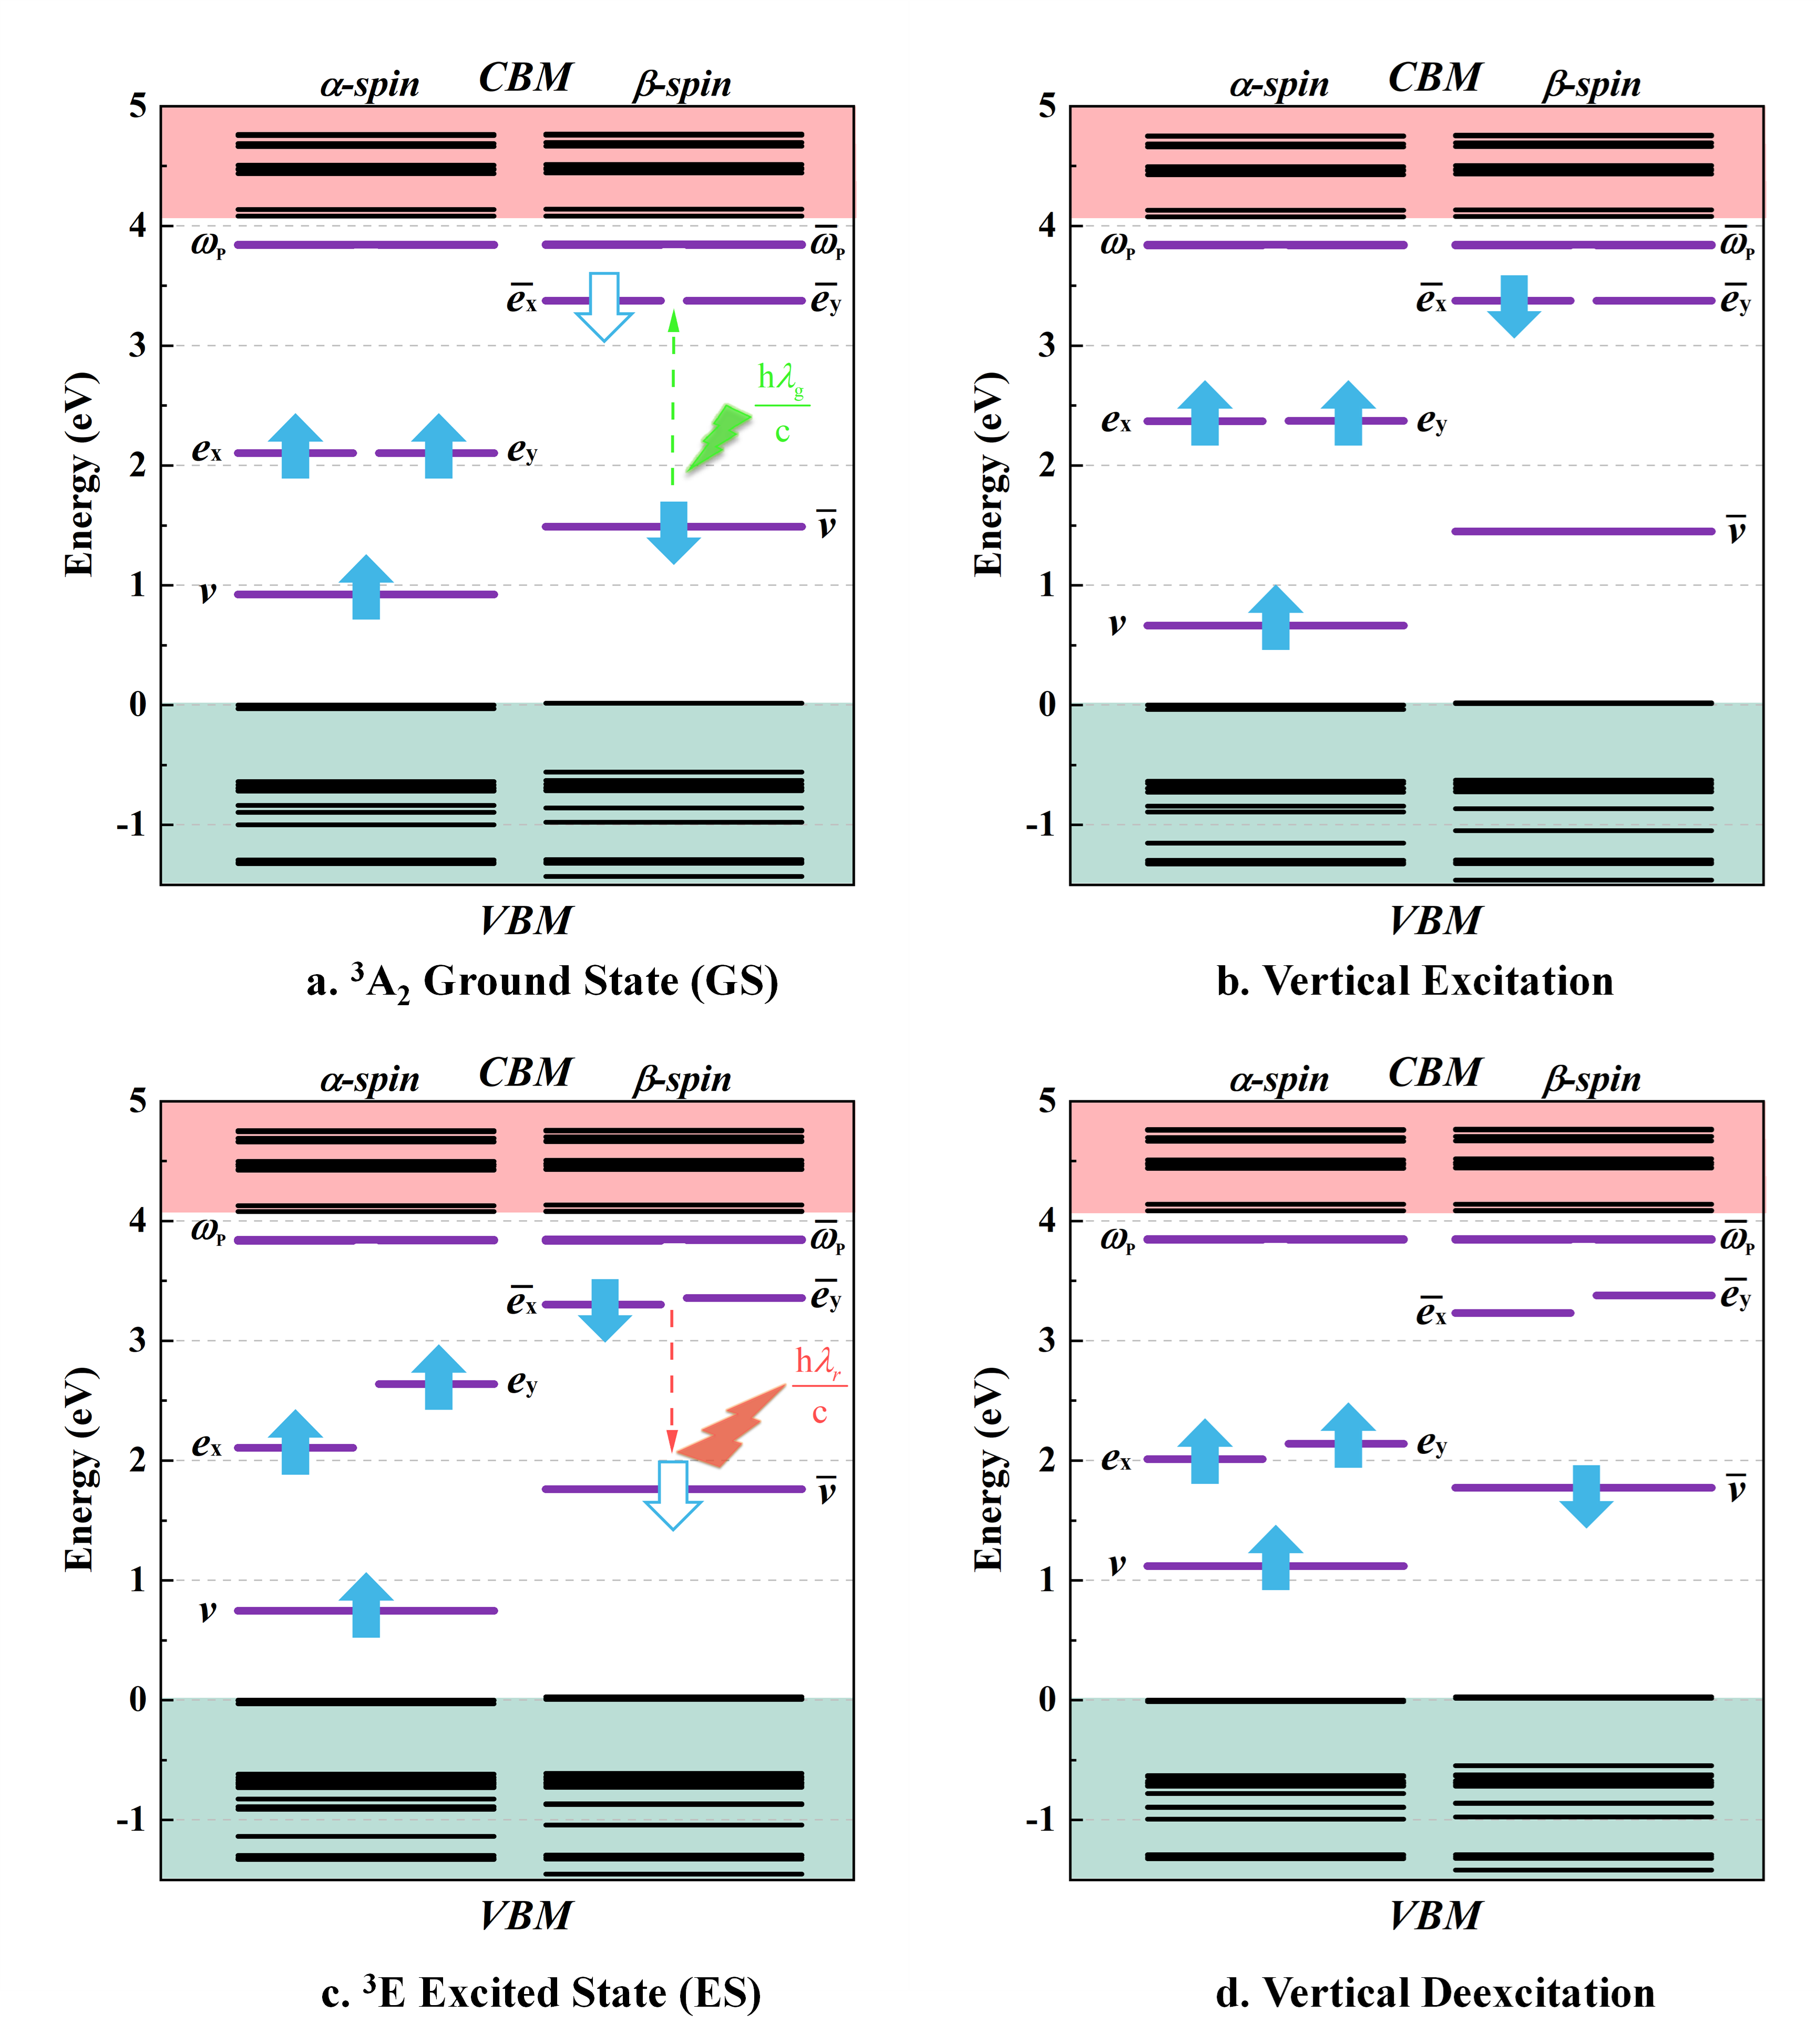
\includegraphics[width=1.0\textwidth]{figures/Chapter 2/Excitation Process.png}
  \caption[ZPL激发过程中电子的能级结构]{ZPL激发过程中电子的能级结构,上下两个区域中填充的浅绿色和粉红色部分分别表示价带最高点(valance band maximum, VBM)和导带最低点(conductive band minimum, CBM)。黑色横线表示价带和导带中不同能级,而中间透明区域中紫色横线表示带隙缺陷能级。分成左右两列绘制了$\alpha$-自旋向上和$\beta$-自旋向下的轨道。蓝色实箭头表示电子占据情况,而空心蓝色箭头表示在$^3A_2$ GS和$^3E$ ES中激发或退激发过程后的电子占据情况。}
  \label{fig: Excitation Process}
\end{figure}

在NV$^-$和NV$^0$的两个光谱曲线中,可以看到声子边带(phonon sidebands, PSB)的作用强度都比ZPL的强度更高,这个过程可以用利用基于Born-Oppenheimer近似和Franck-Condon原理的Huang-Rhys模型来进行简单地描述,即在分子或晶体中,当电子从其基态激发到一个激发态时,会导致与电子激发相关的振动模式被激发。这些振动模式的能级通常称为 "振动激发" 或 "振动副态",而Huang-Rhys 模型用来描述这些振动激发的分布和对电子激发的影响,如图 \ref{fig: Franck-Condon} a\cite{zou2023influence}。在这个模型之中,Huang-Rhys因子$S$决定了晶体结构在基态和激发态之间平衡态位置的差异,这个差异体现了吸收和发射光谱之间的斯托克斯能量位移$E_{Stokes}$。斯托克斯能量唯一和Huang-Rhys因子之间的关系取决于温度,在极低温的时候,光谱曲线中ZPL会有一个较为明显和尖锐的峰值,如图 \ref{fig: Franck-Condon} b所示;而基态和激发态能级之间的能量差异导致的光谱线会随着温度的升高而展宽,一个比较粗略的计算式如下: 
\begin{equation}
  S = (\frac{E_{Stokes}}{2\hbar \omega}+\frac{1}{4})±\frac{1}{4}
\end{equation}
其中$\hbar \omega$代表着缺陷周围晶体的平均声子能量\cite{de2015resolving}。对于NV Center而言,其Huang-Rhys因子在温度较低的情况下的数值一般为2.5 - 5,这表明了激发态相对于基态的结构在空间上有着比较大的偏移,这是两种电荷状态在光谱中决定声子边带形状的关键因素。在ZPL激发的过程中,电子在缺陷能级的占据情况可以通过基于第一性原理的密度泛函理论来计算出来,在仿真的过程中同样遵循Born-Oppenheimer近似和Franck-Condon原理,如图 \ref{fig: Excitation Process}所示,电子在跃迁的过程中保持自旋守恒的状态,仿真是基于Vienna Ab-initio Simulation Package(VASP)软件和杂化泛函Heyd-Scuseria-Ernzerhof (HSE06)算法得到的结果\cite{zou2023influence}。


\begin{figure}
  \centering
  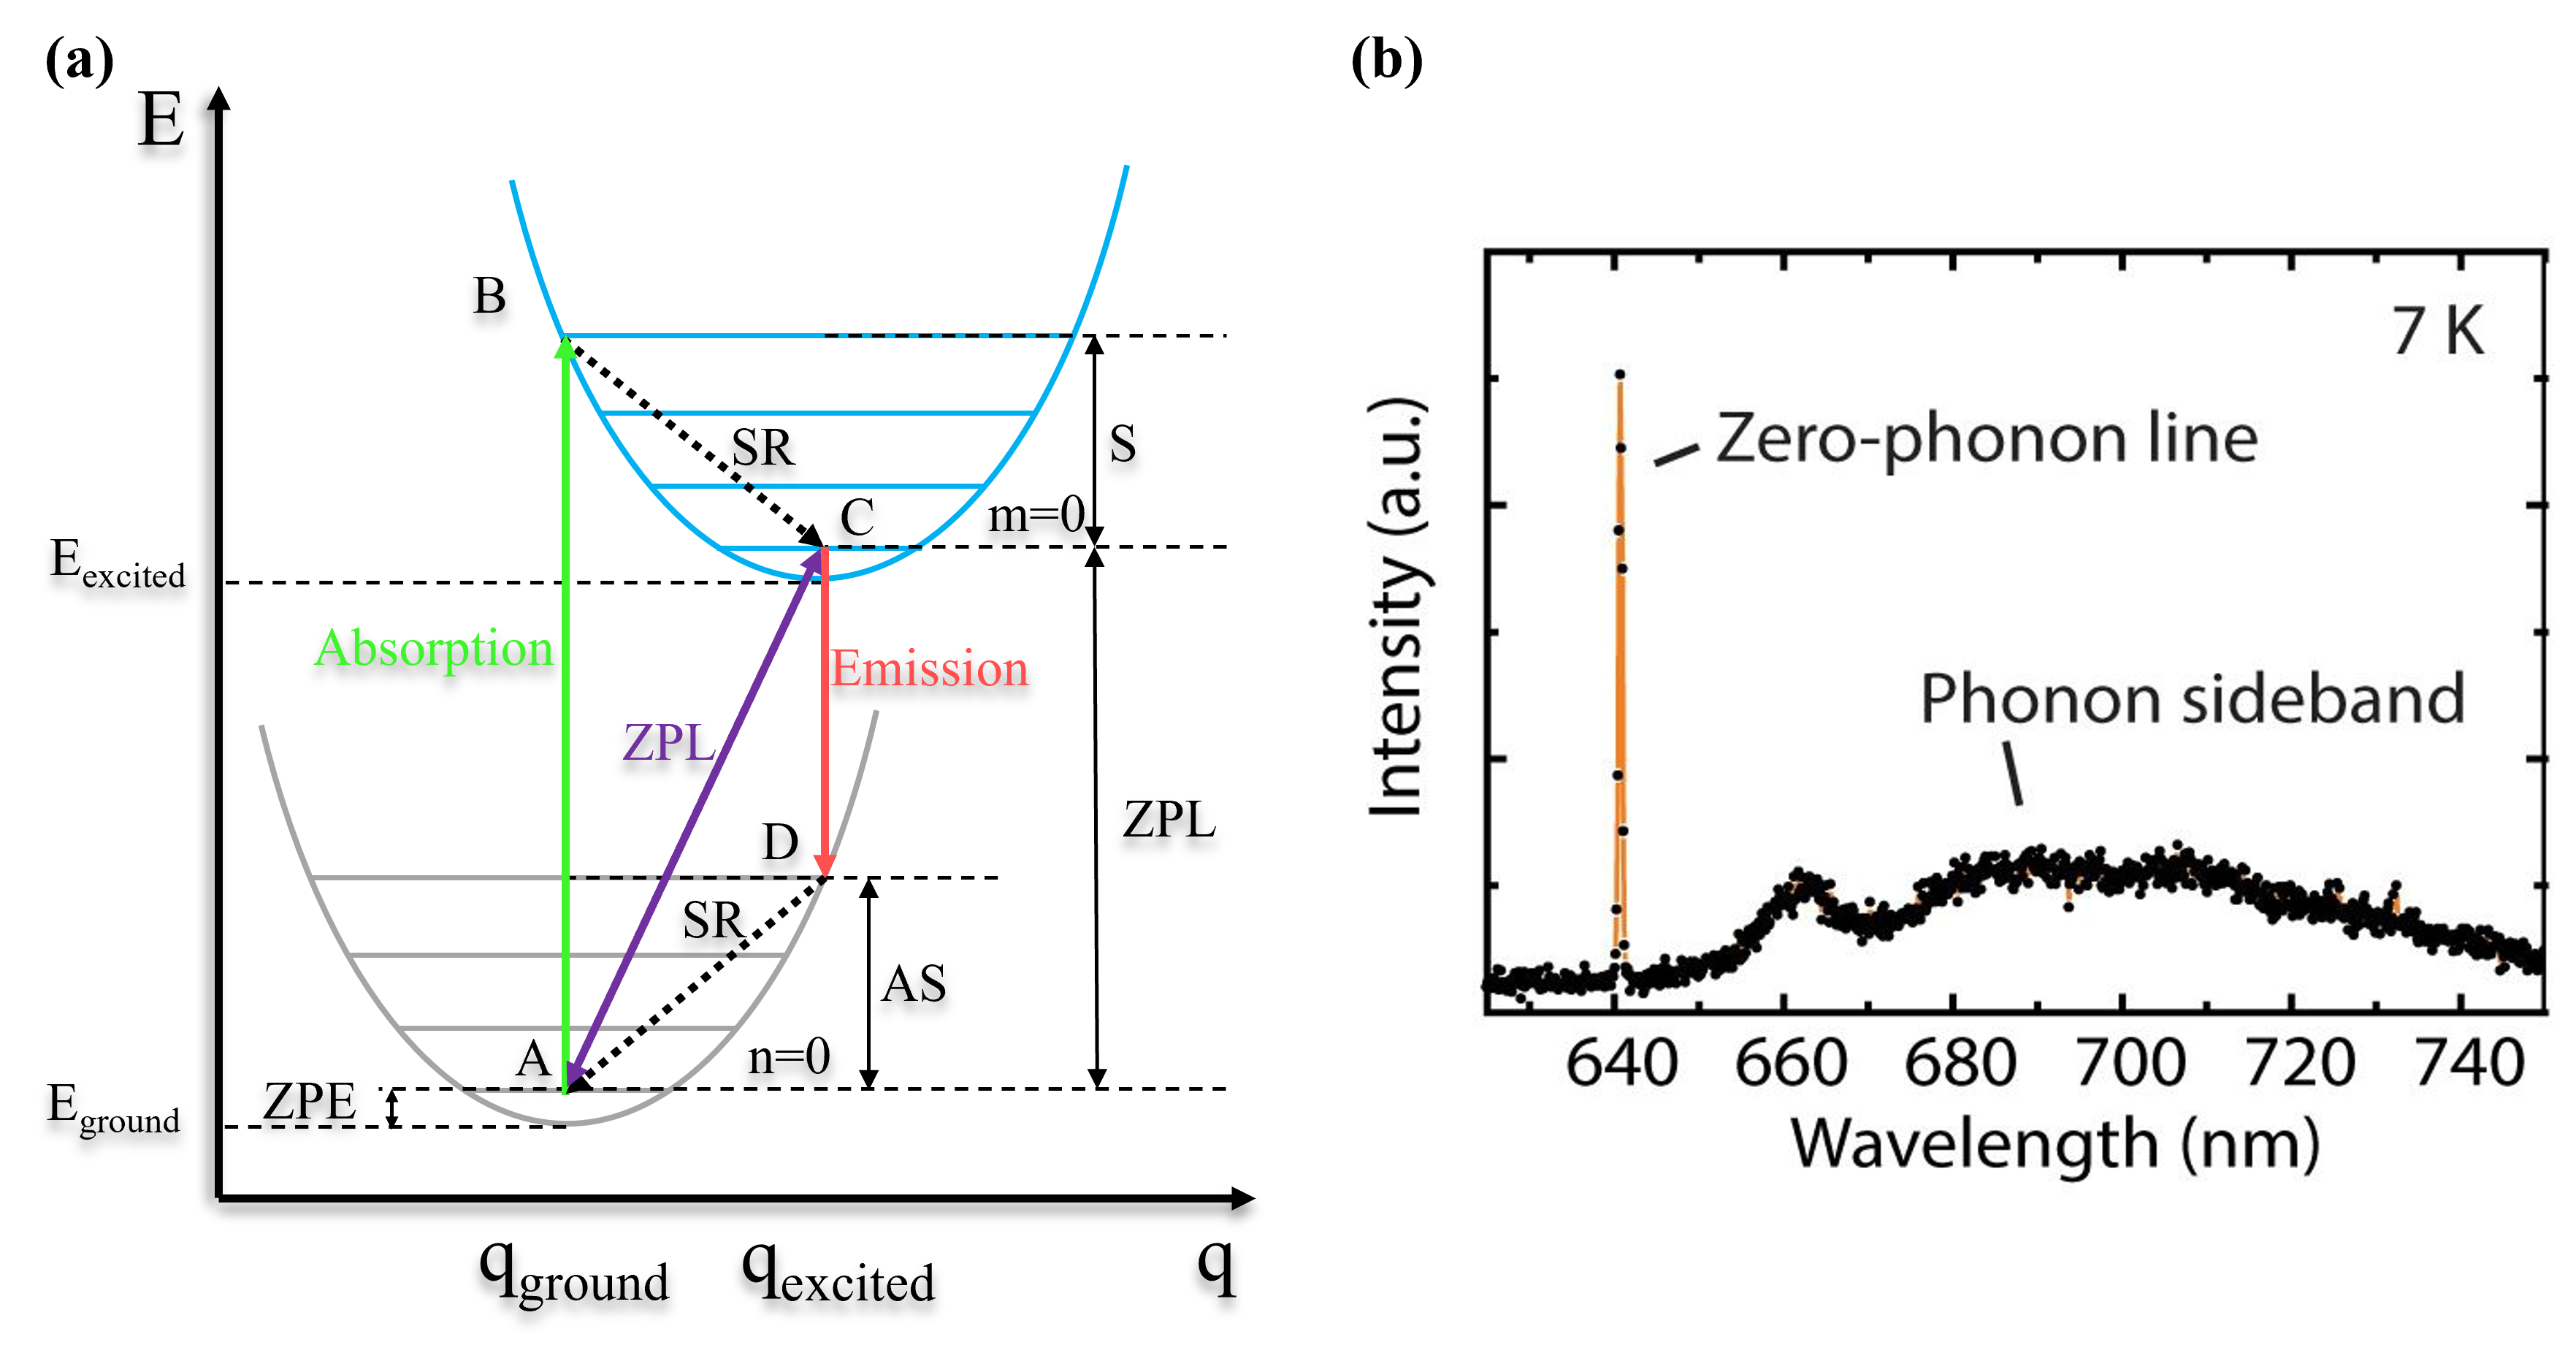
\includegraphics[width=1.0\textwidth]{figures/Chapter 2/Franck-Condon.png}
  \caption[基于Born-Oppenheimer近似和Franck-Condon原理的Huang-Rhys模型示意图]{基于Born-Oppenheimer近似和Franck-Condon原理的Huang-Rhys模型示意图,展示了体系能量(E)和晶体结构坐标(q)的关系。纵轴上的E$_{ground}$和E$_{excited}$分别代表着基态和激发态准抛物线近似能量面的最低能量值,横轴上的q$_{ground}$和q$_{excited}$代表着基态和激发态晶体结构的平衡位置。ZPE为零点能(zero-point energy),最小能量比准抛物线的最低点稍高。}
  \label{fig: Franck-Condon}
\end{figure}

对于本文的工作而言,最重要的是要提高NV$^-$相对于NV$^0$的荧光计数率的比值,所有的计数率都是由基于雪崩光电二极管(Avalanche Photo Diodes, APDs)原理所开发的单光子探测器(Single Photon Detector, SPD)。根据第一章中的图 1.7中所展示的NV$^-$和NV$^0$的光谱曲线的不同,在实验中会在APDs前加入一个650 nm的长通滤光片,这样在收集到的光子中,主要来源则是NV$^-$的荧光发射光子,而NV$^0$的荧光发射的大部分光子则会被滤光片所阻挡。这样,我们就可以通过测量APDs的计数率来判断NV Center的电荷态,从而可以对NV Center的电荷态进行观测和表征。

单光子激发NV Center从基态跃迁到激发态然后退激发的荧光过程中,激发态有一定的寿命,这个寿命和其周围金刚石晶体的声子的活跃性有关,在寿命时间之后,激发态会自发地退激发到基态,这个过程会伴随着荧光光子的发射,发射出的光子波长和其能量有关,而能量则取决于跃迁能量和声子在激发过程中的振动能量。由于这是一个单光子过程,所以在较低的激发激光的功率下,两种电荷态的荧光计数率和光强是成线性的关系,也就是激光功率决定了可以到达NV Center并参与激发过程的光子的数量\cite{aslam2013photo}。对于单个NV Center而言,其可以作为光子发射的结构,由于激发态有一定的寿命,所以发射的荧光强度随着激发光强的提高,会出现饱和的现象。在激发光强超过饱和光强$P_{Sat}$的时候,NV Center的荧光强度将不再明显地增加,拟合公式为:
\begin{equation}
  F \propto N_2 +AP = C \frac{P/P_{Sat}}{1+P/P_{Sat}}+AP
\end{equation} 
其中$F$为单光子探测器单位时间内的读数,$N_2$为激发态布居数,$P$为当前激光强度,$P_{Sat}$为饱和激光强度,$AP$为激光漏光进入单光子探测器的读数,其数值正比于激光强度,通常情况下拟合曲线如图 \ref{fig: Saturation Plot}所示,从图中可以看出其饱和激发光强是854.86 \unit{\uW},该光强下的NV Center荧光发光的计数率为70.21 kpcs/s。金刚石表面的吸收和散射会导致激光功率的损失,所以在制备样品的过程中,我们在金刚石表面设计了纳米立柱(nano pillar)结构,然后将氮离子注入其中,再退火形成位于nano pillar结构中NV Center,如图 \ref{fig: nano pillar}。

\begin{figure}
  \centering
  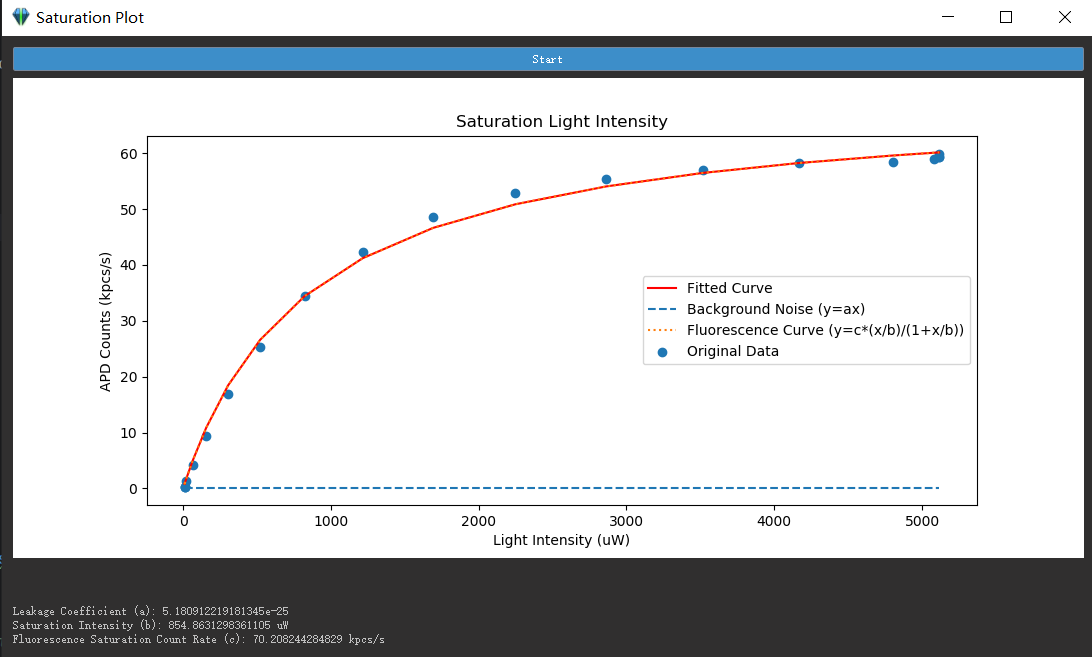
\includegraphics[width=1.0\textwidth]{figures/Chapter 2/Saturation Plot.png}
  \caption[单个NV Center光强饱和曲线]{单个NV Center光强饱和曲线,横轴是激发光强,纵轴是APDs计数率,图中展示了饱和激发光强的大小和该情况下NV Center荧光发光的计数率。}
  \label{fig: Saturation Plot}
\end{figure}

\begin{figure}
  \centering
  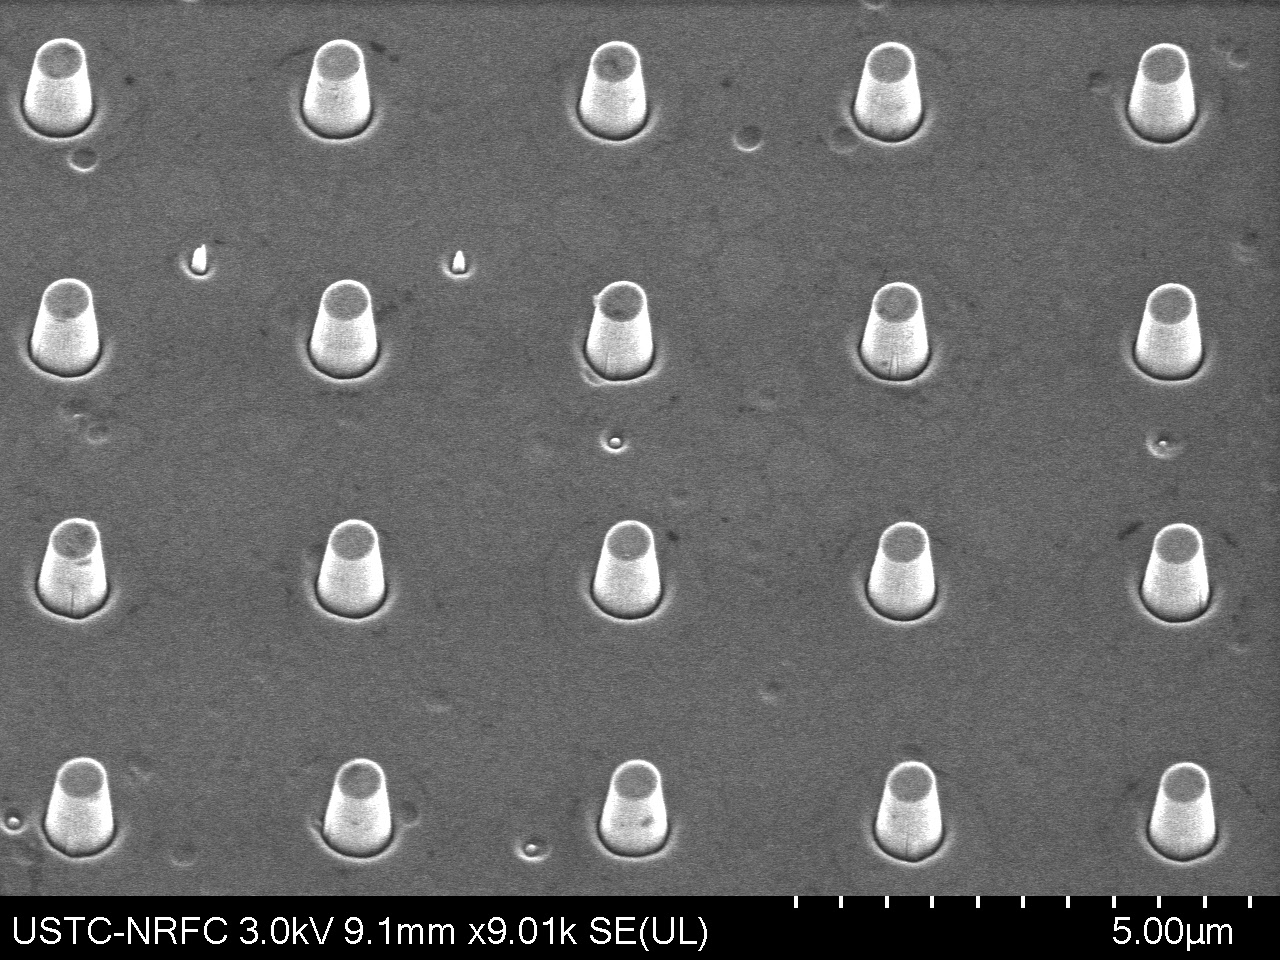
\includegraphics[width=1.0\textwidth]{figures/Chapter 2/nano pillar.png}
  \caption[金刚石表面nano pillar结构]{金刚石表面nano pillar结构}
  \label{fig: nano pillar}
\end{figure}

\subsection{NV Center电荷态之间的电离和复合过程}
对于NV Center的两种电荷态NV$^-$和NV$^0$,它们之间有相互转换的机制,即缺陷能级电子的电离和复合(ionization and recombination)的过程,如图 \ref{fig: Ionization and Recombination}所示。

图 \ref{fig: Ionization and Recombination}a和b展示了从NV$^-$到NV$^0$的电离过程。在这个过程中,第一个光子激发NV$^-$基态能级的电子到激发态,紧接着第二个光子激发同一个电子,使其从带隙中的缺陷能级激发到金刚石导带能级,这让NV Center成为仅有一个未成对电子的电中性NV$^0$状态。图 \ref{fig: Ionization and Recombination}c和d展示了从NV$^0$到NV$^-$的复合过程,一个电子从NV$^0$自旋双重态的基态跃迁到激发态,和金刚石价带中的一个激发的电子结合,从而使得缺陷能级中重新拥有两个未成对的电子,回到负电的NV$^-$状态。

\begin{figure}
  \centering
  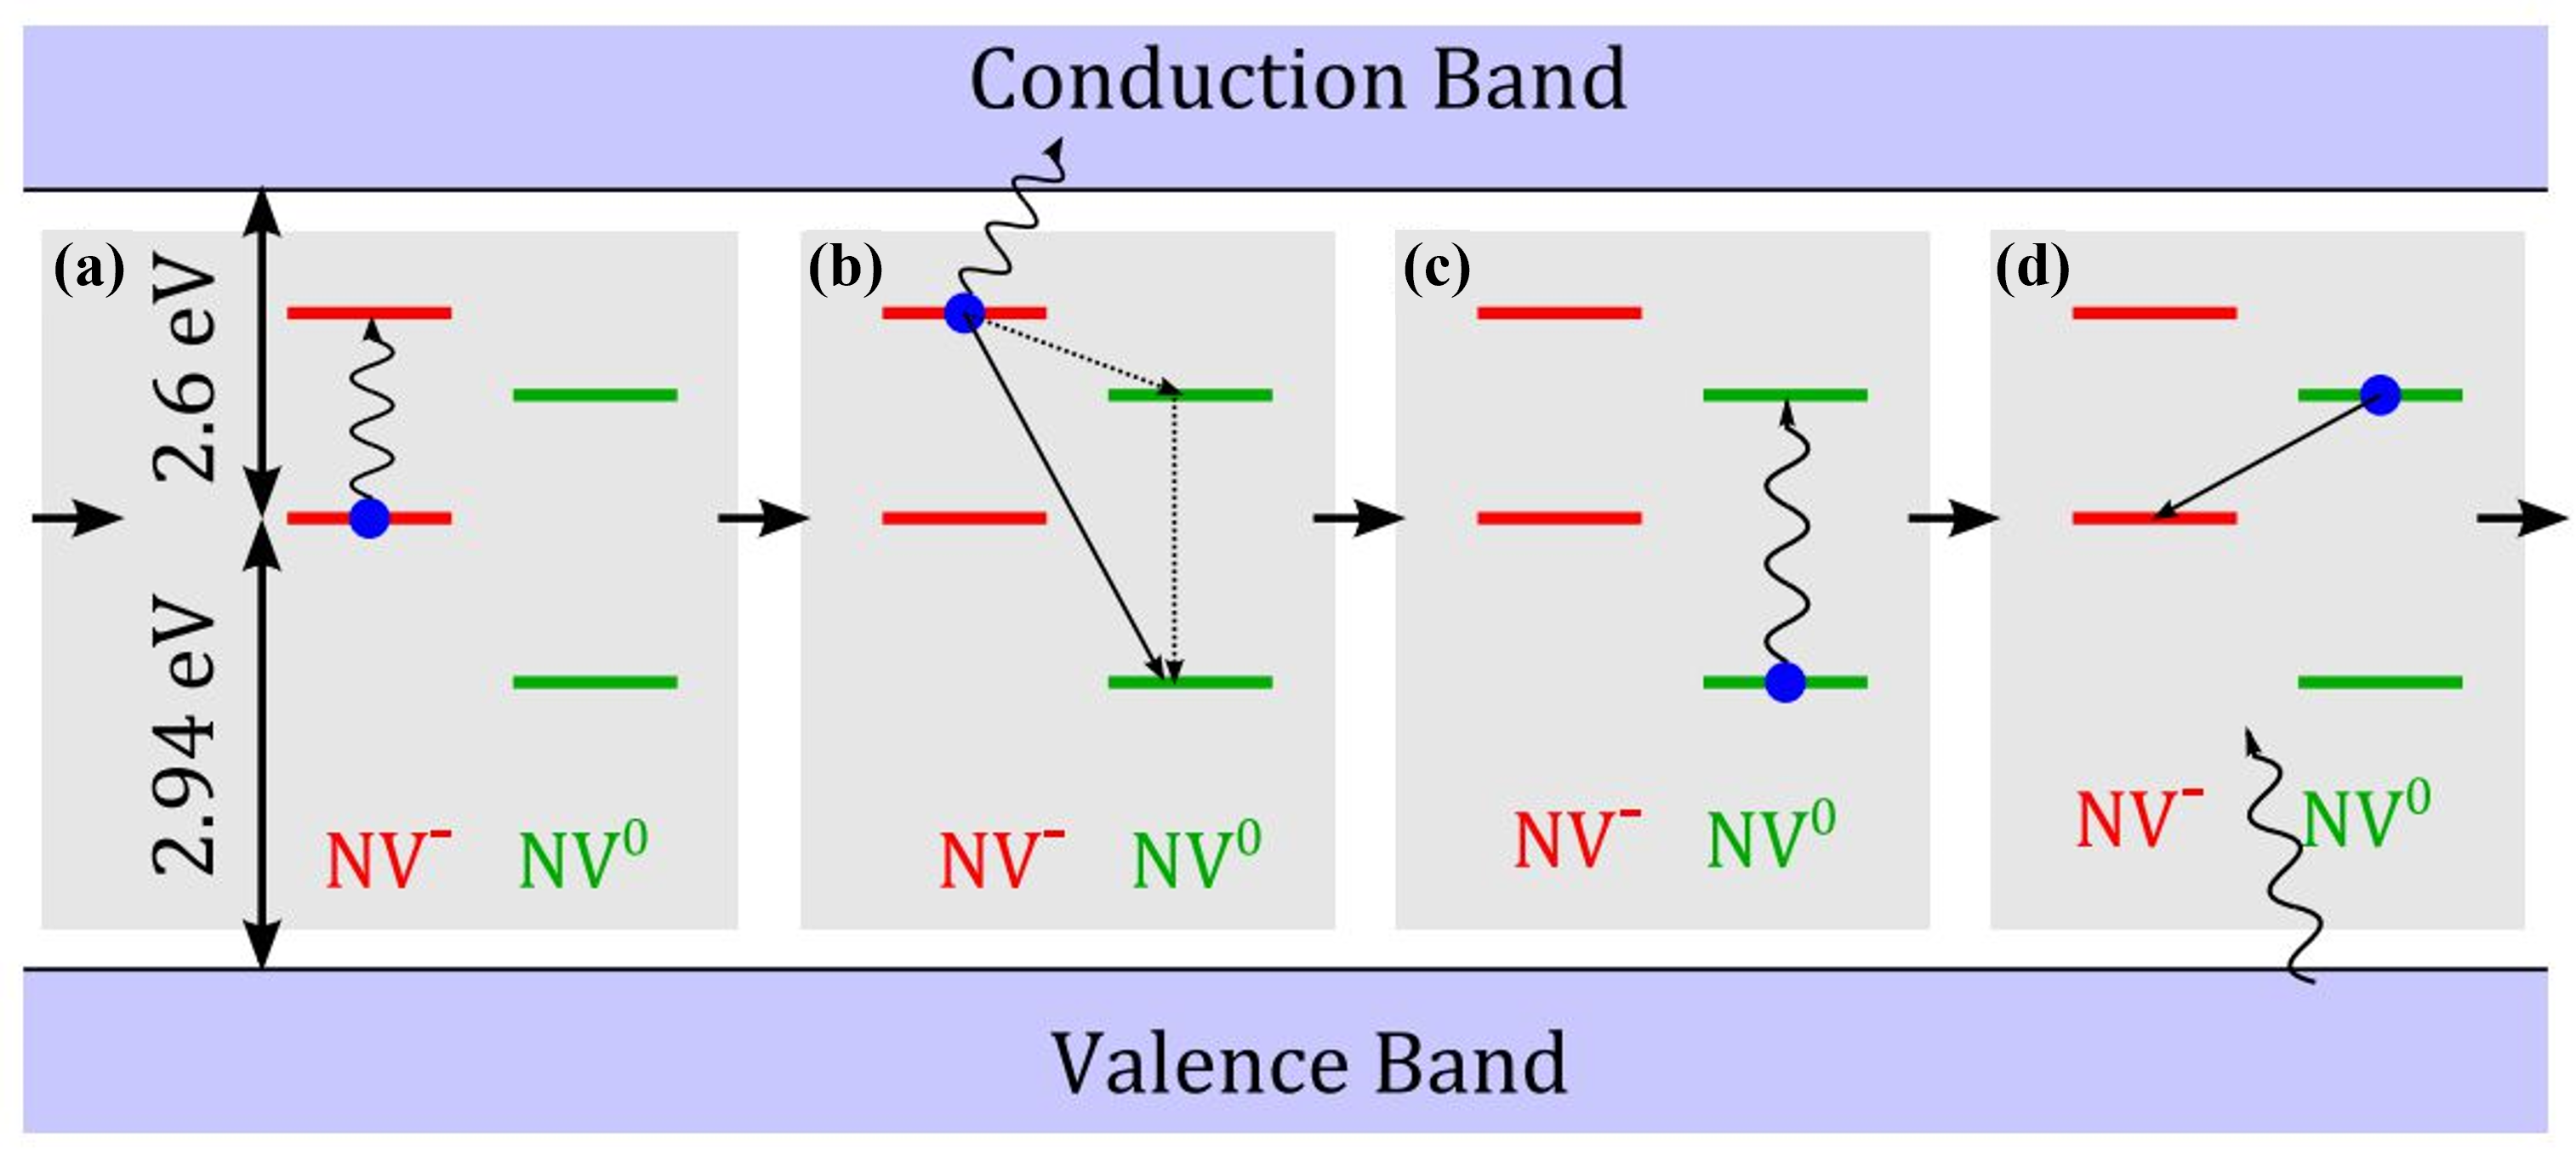
\includegraphics[width=1.0\textwidth]{figures/Chapter 2/Ionization and Recombination.png}
  \caption[NV Center带隙中缺陷能级电子的电离和复合过程]{NV Center带隙中缺陷能级电子的电离和复合过程\cite{aslam2013photo}。}
  \label{fig: Ionization and Recombination}
\end{figure}

不论是电离还是复合的过程,光电子的动力学特征都极其依赖于激光的波长,如图 \ref{fig: Different Wavelength}。因此,当激发光路波长在637 nm的时候,NV Center中的NV$^-$的占比将会随着时间急剧下降,即被电离为NV$^0$;532 nm的激发光子会将NV Center的电荷态向着NV$^-$占比更高的方向进行初始化。而本文中最重要的一个调控方式就是利用594 nm波长的黄橙光来抑制中性的NV$^0$结合电子从而复合成负电中心的NV$^-$。在这个激发的条件下,NV$^-$基态处于$m_s = 0, ±1$的电子都会被激发到激发态。由于存在ISC过程,之前处于基态$m_s = ±1$的电子会落到自旋单态的能级,而之前处于基态$m_s=0$的电子则会回到激发态$m_s=0$能级。然后功率较高的637 nm激光快速脉冲使得这些处于激发态$m_s=0$能级的电子激发到金刚石晶体的导带,从而使得NV Center呈现NV$^0$的电中性状态,而此时处于自旋单态的电子回到基态$m_s=0$的能级,这样使得将NV$^-$的自旋分布情况转换成可以读出的电荷分布状态。最后利用较低功率的594 nm的激光对这些回到基态$m_s=0$的能级的自旋状态进行长时间的读出并记录,通过荧光效应来观测并推导出电荷态的分布,通过APDs计数率的变化可以明显的看到这一过程,在594 nm激光连续波(continuous wave, CW)的持续作用下,我们可以观测到NV$^-$(高计数率)和NV$^0$(低计数率)之间存在一个特定的比例关系\cite{waldherr2011dark}。在这里,我们之所以使用594 nm的橙光来进行读出,是因为这个波长的光子能量比532 nm的能量稍低,可以防止将NV$^0$的电子激发,使之和价带电子结合,从而回到NV$^-$的状态,这样就将NV$^0$的状态保护了起来,便于读出信息,而不会像532 nm的光子会将NV Center初始化到NV$^-$的$m_s=0$。ll

\begin{figure}
  \centering
  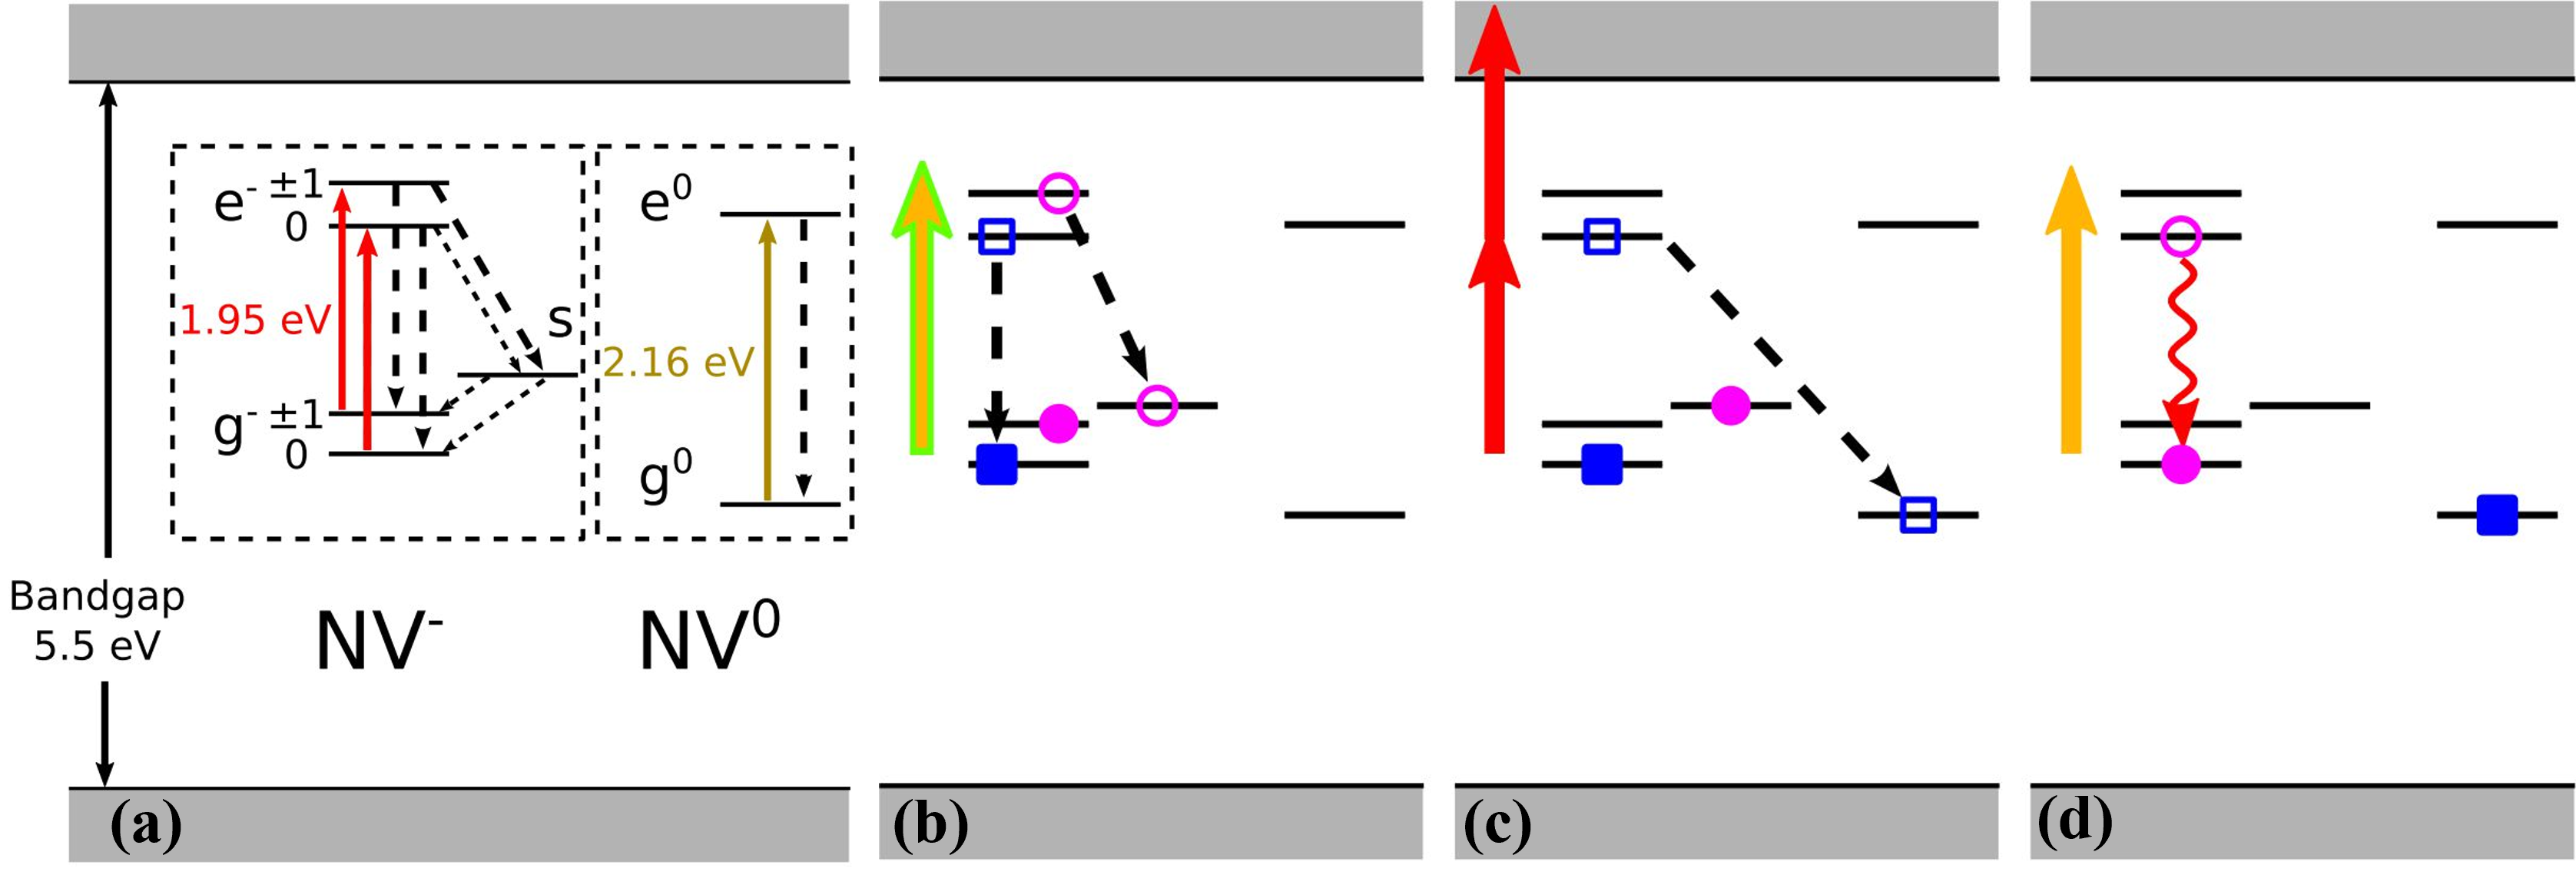
\includegraphics[width=1.0\textwidth]{figures/Chapter 2/Different Wavelength.png}
  \caption[NV$^-$和NV$^0$的电子能级结构和不同波长激光对于电子的调控]{NV$^-$和NV$^0$的电子能级结构和不同波长激光对于电子的调控,a、b、c分别是532 nm的绿光(或594 nm的黄橙光)、637 nm的红光、594 nm的黄橙光\cite{shields2015efficient}。}
  \label{fig: Different Wavelength}
\end{figure}

这些现象表明,NV Center的电荷态随着时间的变化并不是一个稳定的情况,而是有一个动态变化的状态,可以通过随着时间变化的相对电离和复合率来描述,这也是本文主要聚焦的问题。由于电离和复合的过程都可以用双光子过程来描述,因此在激光功率较低的时候,NV Center的荧光效应没有饱和前,电离和复合和激光光强有关,在后续的分析中需要考虑饱和光强这一限制因素。

除此之外,NV Center电荷态的电离和复合过程同样受到环境的影响,包括样品的晶体结构、掺杂等因素,以及环境温度、磁场、电场等实验环境因素,这些会在没有任何荧光效用的情况下影响NV Center的电荷态。比如,在制备样品的过程中,金刚石晶体中的一些缺陷结构会形成局域电子势阱(local electron traps),在NV$^-$转化为NV$^0$之后停止光学激发,电子将不会回落到NV Center缺陷能级附近,使得其变为暗态\cite{bluvstein2019identifying}。除此之外,一些施主掺杂元素在没有外界激发的激发的情况下,也会在一定程度上影响NV$^-$的布局数分布\cite{doi2016pure}。本人也曾利用基于第一性原理的密度泛函理论探究并证明了相比于实验中最为常见的氮元素施主掺杂的金刚石中的NV Center而言,磷元素施主掺杂的金刚石中的NV$^-$在保证其原有的量子比特的各种优异性质的同时,其NV Center的负电中心稳定性更强\cite{zou2023influence}。

\section{NV Center电荷态动力学的理论模型}
在这一部分,本文将基于B. J. Shields和L. Hacquebard等人提出的方案,对于NV Center电荷态动力学的理论模型进行构建和分析\cite{shields2015efficient, hacquebard2018charge}。NV Center的荧光发光特征可以通过在时间尺度记录APDs所收集到的单光子计数率来表征,当NV Center处于NV$^-$状态的时候,会有较高的计数率$\gamma_-$;当NV Center处于NV$^0$状态的时候,会有较低的计数率$\gamma_0$。$\gamma_-$和$\gamma_0$在本文后续都分别指代NV$^-$和NV$^0$的计数率,并用这两个可以直接探测到的参数在特定的读出时间(readout time)$t_r$区间下来构建收集到光子数结果的直方图。如果在一定的读出时间$t_r$之中,NV Center的电荷态没有发生改变,那这个可以用两个泊松概率分布函数(Poissonian Probability Distribution Functions, PPDF)来分别描述NV$^0$和NV$^0$态的布居数分布直方图:
\begin{equation}
  PPDF_0(n, \gamma_0 t_r) = \frac{(\gamma_0 t_r)^n exp(-\gamma_0 t_r)}{n!}
  \label{equ: PPDF_0}
\end{equation}
\begin{equation}
  PPDF_-(n, \gamma_- t_r) = \frac{(\gamma_- t_r)^n exp(-\gamma_- t_r)}{n!}
  \label{equ: PPDF_1}
\end{equation}
由于计数率的单位与时间相关,通常为kpcs/s(千光子每秒),而且荧光的光子在特定的读出时间中是随机的统计分布,也就是在自然情况下遵循泊松分布,即所以读取到特定电荷态计数率的均值为$\gamma_0 t_r$或$\gamma_- t_r$,作为泊松分布函数的变量,因此在一定的读出时间$t_r$之中,探测到的光子数量$n$的直方图可以计算:
\begin{equation}
P_{hist}(n)=P(NV^0)PPDF_0(n, \gamma_0 t_r)+P(NV^-)PPDF_-(n, \gamma_- t_r)
\end{equation}
其中$P(NV^0)$和$P(NV^-)$是在读出时间$t_r$的开始,NV Center处于特定电荷态的概率,两种状态的初始概率分别由单个泊松分布在总面积中占据的比例决定的。

然而,前文所讨论的NV Center缺陷电子能级结构中,未成对电子的电离和复合对应的电荷态的转换及其过程中的荧光效应的描述是一个简化模型,实际上电荷态在读出时间的尺度之内是极其不稳定的,可能会在这个时间段内发生数次电荷态的转换,这种电荷态转换可以用从NV$^0$到NV$^-$的复合率$g_{0-}$和从NV$^-$到NV$^0$的电离率$g_{-0}$这两个参数来描述。为了简单理解这样的电荷态动态转化的过程,可以用一些简单的例子来说明,如图 \ref{fig: Charge Conversion}a所示。在这个$t_r$的过程中,初始的电荷态为NV$^0$,持续时间为$\tau_1$,然后复合形成NV$^-$的概率为:
\begin{equation}
  p_1(\tau_1,g_{0-}) = g_{0-}\tau_1 \cdot e^{-g_{0-}\tau_1}
\end{equation}
这个式子为PPDF公式\ref{equ: PPDF_0}简单形式,其中$n=1$,$\gamma_0 = g_{0-}$,$t_r=\tau_1$。
同样的,对于序列的第二段和第三段而言,其概率为:
\begin{equation}
  p_2(t_1,g_{-0}) = g_{-0}t_1 \cdot e^{-g_{-0}t_1}
\end{equation}
\begin{equation}
  p_3(\tau_2,g_{0-}) = \tau_2 \cdot e^{-g_{0-}\tau_2}
\end{equation}
需要注意的是,我们假设在第三部分后,不会有电荷转换的情况产生,所以系数中不存在$g_{0-}$这一项。对于时间而言,有$\tau=\tau_1+\tau_2$和$t_r-\tau=t_1$,所以整体的概率为上述三个概率的乘积:
\begin{equation}
  \begin{aligned}
    P_a(\tau,t_r,g_{0-},g_{-0}) &= p_1 \cdot p_2 \cdot p_3 \\
    &= g_{0-}g_{-0}\tau_1\tau_2t_1 \cdot e^{(g_{-0}-g_{0-})\tau-g_{-0}t_r}
  \end{aligned}
\end{equation}
同样的,对于另外三种可能的情况,概率计算的结果如下:
\begin{equation}
  P_b(\tau,t_r,g_{0-},g_{-0}) = g_{-0}g_{0-}\tau_1\tau_2t_1 \cdot e^{(g_{0-}-g_{-0})\tau-g_{0-}t_r}
\end{equation}
\begin{equation}
  P_c(\tau,t_r,g_{0-},g_{-0}) = g_{0-}\tau_1t_1 \cdot e^{(g_{-0}-g_{0-})\tau-g_{-0}t_r}
\end{equation}
\begin{equation}
  P_c(\tau,t_r,g_{0-},g_{-0}) = g_{-0}\tau_1t_1 \cdot e^{(g_{0-}-g_{-0})\tau-g_{0-}t_r}
\end{equation}

\begin{figure}
  \centering
  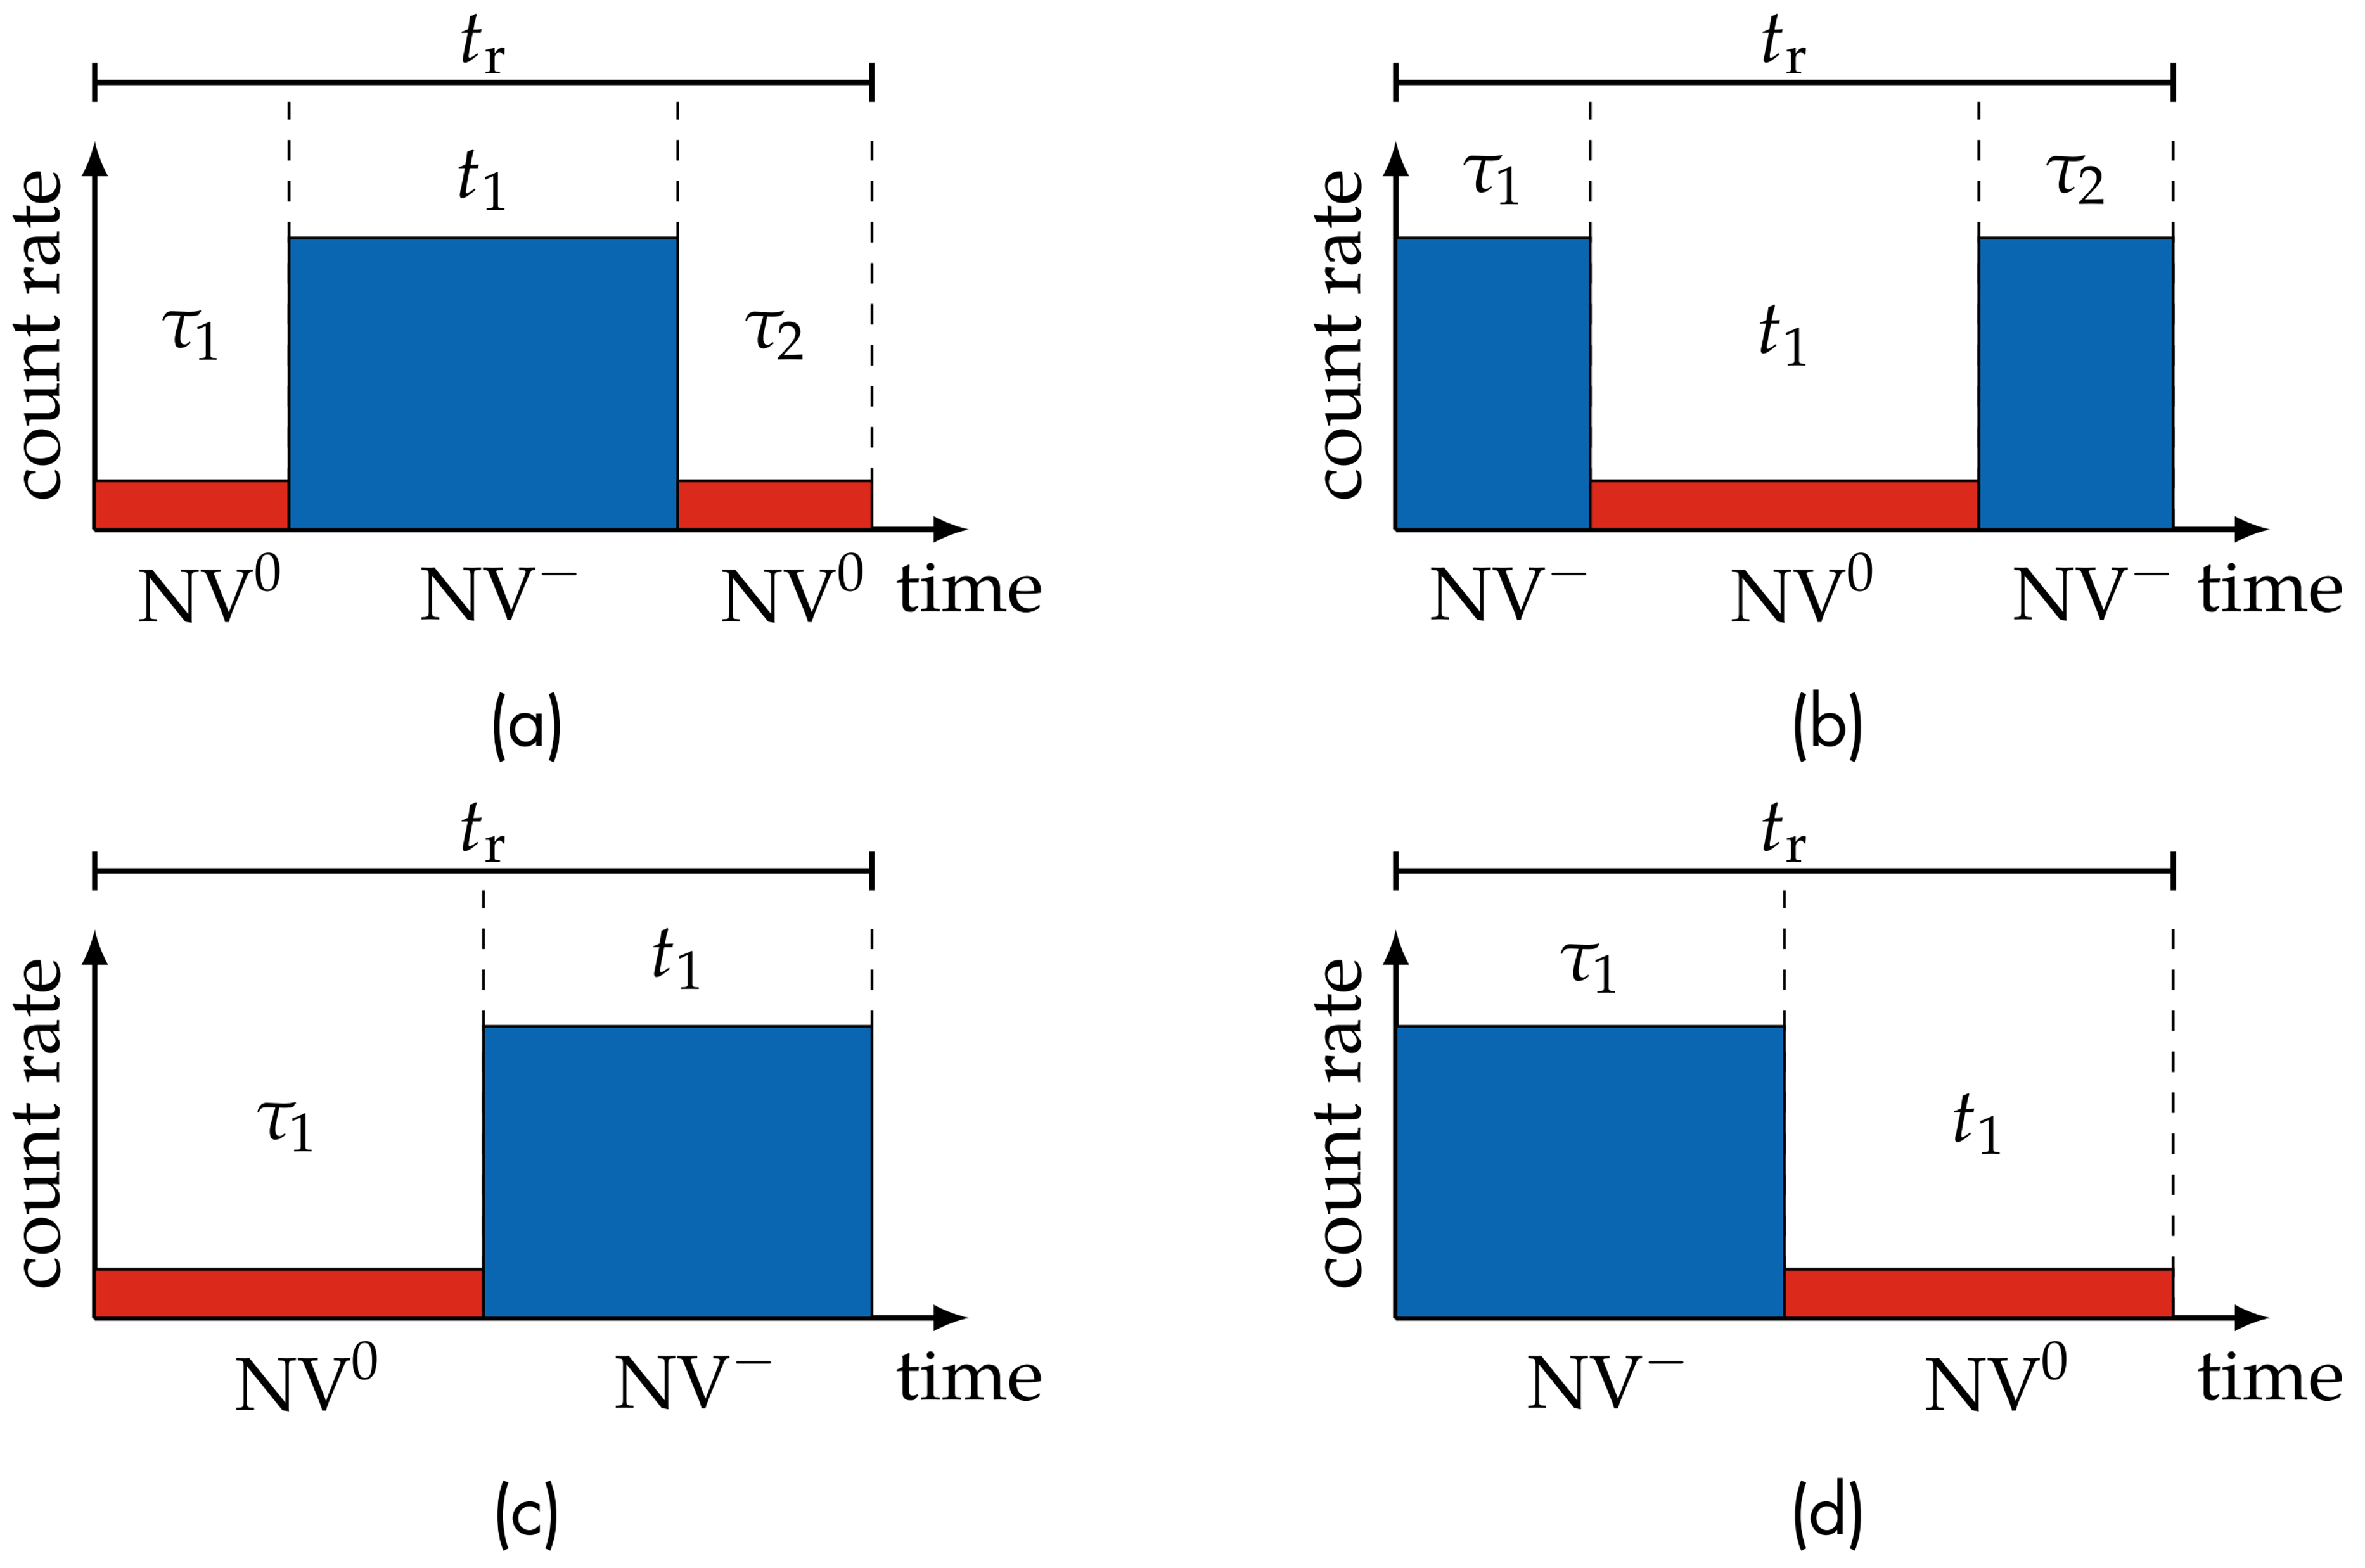
\includegraphics[width=1.0\textwidth]{figures/Chapter 2/Charge Conversion.png}
  \caption[不同电荷初态时,NV Center电荷态的转换过程示意图]{不同电荷初态时,NV Center电荷态的转换过程示意图,观测的时间尺度为读出时间$t_r$, $\tau_i$为在$t_r$中和初始电荷态相同状态所持续的时间,$t_i$为在$t_r$中和初始电荷态不同状态所持续的时间。(a)初始电荷态为NV$^0$,且电荷态的转换次数为偶数;(b)初始电荷态为NV$^-$,且电荷态的转换次数为偶数;(c)初始电荷态为NV$^0$,且电荷态的转换次数为奇数;(d)初始电荷态为NV$^-$,且电荷态的转换次数为奇数。}
  \label{fig: Charge Conversion}
\end{figure}

在图 \ref{fig: Charge Conversion}中所展示的是在读出时间$t_r$中最基本的四种序列,分类依据是初始电荷态是NV$^-$或者NV$^0$以及电荷态转换的次数是奇数次或者偶数次。更一般的情况下,可以将这些情况进行组合,并且可能会有很多次的电荷态转换的现象产生,所以可以写出更为普适性的表达式,即对上面推导的式子分情况进行积分和求和:
\begin{equation}
  \begin{aligned}
    p(n|NV^0,even)=&\int_{0}^{t_r}d\tau e^{(g_{-0}-g_{0-})\tau-g_{-0}t_r} \sum_{i=1}^{\infty}(g_{0-}g_{-0})^i \prod_{j=1}^{i}\int_{0}^{\tau-\sum_{k=1}^{j-1}\tau_k}d\tau_j \\
    & \times \prod_{j=1}^{i-1}\int_{0}^{(t_r-\tau)-\sum_{k=1}^{j-1}t_k}dt_jPPDF(n, \gamma_0\tau+\gamma_-(t_r-\tau)) \\
    & + e^{-g_{0-}t_r}PPDF(n, \gamma_0t_r)
  \end{aligned}
\end{equation}
\begin{equation}
  \begin{aligned}
    p(n|NV^-,even)=&\int_{0}^{t_r}d\tau e^{(g_{0-}-g_{-0})\tau-g_{0-}t_r} \sum_{i=1}^{\infty}(g_{-0}g_{0-})^i \prod_{j=1}^{i}\int_{0}^{\tau-\sum_{k=1}^{j-1}\tau_k}d\tau_j \\
    & \times \prod_{j=1}^{i-1}\int_{0}^{(t_r-\tau)-\sum_{k=1}^{j-1}t_k}dt_jPPDF(n, \gamma_-\tau+\gamma_0(t_r-\tau)) \\
    & + e^{-g_{-0}t_r}PPDF(n, \gamma_-t_r)
  \end{aligned}
\end{equation}
\begin{equation}
  \begin{aligned}
    p(n|NV^0,odd)=&\int_{0}^{t_r}d\tau e^{(g_{-0}-g_{0-})\tau-g_{-0}t_r} \sum_{i=1}^{\infty}g_{0-}^ig_{-0}^{i-1} \prod_{j=1}^{i-1}\int_{0}^{\tau-\sum_{k=1}^{j-1}\tau_k}d\tau_j \\
    & \times \prod_{j=1}^{i-1}\int_{0}^{(t_r-\tau)-\sum_{k=1}^{j-1}t_k}dt_jPPDF(n, \gamma_0\tau+\gamma_-(t_r-\tau)) \\
    & + e^{-g_{0-}t_r}PPDF(n, \gamma_0t_r)
  \end{aligned}
\end{equation}
\begin{equation}
  \begin{aligned}
    p(n|NV^-,odd)=&\int_{0}^{t_r}d\tau e^{(g_{0-}-g_{-0})\tau-g_{0-}t_r} \sum_{i=1}^{\infty}g_{-0}^ig_{0-}^{i-1} \prod_{j=1}^{i-1}\int_{0}^{\tau-\sum_{k=1}^{j-1}\tau_k}d\tau_j \\
    & \times \prod_{j=1}^{i-1}\int_{0}^{(t_r-\tau)-\sum_{k=1}^{j-1}t_k}dt_jPPDF(n, \gamma_-\tau+\gamma_0(t_r-\tau)) \\
    & + e^{-g_{-0}t_r}PPDF(n, \gamma_-t_r)
  \end{aligned}
\end{equation}
这四个通用公式是由M. D. Lukin及其团队在2015年提出的,用以解释电荷态在一定的读出时间内转换的普适性概率模型 \ref{shields2015efficient}。由这个公式,我们可以得到在这个读出时间段内光子数$n$的直方图计算表达式:
\begin{equation}
  \begin{aligned}
    P(n)&=P(NV^0)[p(n|NV^0,even)+p(n|NV^0,odd)] \\
    &+P(NV^-)[p(n|NV^-,even)+p(n|NV^-,odd)] \\
    &=P(NV^0)p(n|NV^0)+P(NV^-)p(n|NV^-)
  \end{aligned}
\end{equation}
由这个式子可以得到,在这个模型中,只剩下初始态处于NV$^0$或NV$^-$的概率$P(NV^0)$和$P(NV^-)$需要来确定,由此我们需要进行连续波(continuous wave)和脉冲(pulsed)测量来分布确定所需要的数据,这里的连续波和脉冲测量指的是在读出时间内激光是否会间断。

\subsection{CW测量下初始电荷态分布和读出保真度}
一旦知道了电荷态转换率$g_{-0}$和$g_{0-}$,电荷态动力学分布就可以用下面两个微分系统方程来描述:
\begin{equation}
  \dot{\rho}_- = g_{0-}\rho_0-g_{-0}\rho_-
  \label{equ: differential equations_-}
\end{equation}
\begin{equation}
  \dot{\rho}_0 = -g_{0-}\rho_0+g_{-0}\rho_-
  \label{equ: differential equations_0}
\end{equation}
其中$\rho_-$是负电荷态总体概率分布,而$\rho_0$是中性电荷态总体分布的概率,即:
\begin{equation}
  P(NV^-) \equiv \rho_-
\end{equation}
\begin{equation}
  P(NV^-) \equiv 1-\rho_- = \rho_0
\end{equation}
然而,在恒定功率和波长的激光CW激发测量下,系统中的电荷态是近乎稳定,也就是$\dot{\rho}_0 = \dot{\rho}_- = 0$,因此由式\ref{equ: differential equations_-}和\ref{equ: differential equations_0}可以得到:
\begin{equation}
  \frac{g_{0-}}{g_{-0}}=\frac{\rho_-}{\rho_0}
\end{equation}
\begin{equation}
  P(NV^-)=\frac{g_{0-}}{g_{0-}+g_{-0}}
\end{equation}
通过这些计算,可以构建利用CW测量电荷态的模型和实验方案。

另外一个比较重要的特征是我们可以通过CW测量来得到读出保真度$\mathcal{F}_C$,也就是我们能够顺利读出并正确判断电荷态的可信度。其中一个关键点是设定一个合适的光子计数率阈值$n_{thresh}$来区分NV$^0$和NV$^-$的分布状态。因为NV$^0$状态时的计数率要远低于NV$^-$,所以在一定的读出时间$t_r$之中,如果计数率低于$n_{thresh}$,则计入NV$^0$的部分,反之则计入NV$^-$的部分。读出效率的公式可以由此计算:
\begin{equation}
  \mathcal{F}_c = \frac{1}{2}[\sum_{n=0}^{n_{thresh}}p(n|NV^0)+\sum_{n_{thresh}}^{n_{max}}p(n|NV^-)]
\end{equation}
我们需要最大化读出效率,所以需要对于读出594 nm橙光的功率$P$和读出时间$t_r$进行测试和优化,从而使得$\mathcal{F}_C$达到尽可能大的数值,这对于基于单次读出激光来收集统计光子数的单次读出(single shot readout)技术而言非常重要。

除此之外,区分NV$^0$和NV$^-$的阈值$n_{thresh}$的设定同样十分重要。如图 \ref{fig: n_thresh}所示,左图(a)为实验中利用APDs测得的原始数据,展示了在读出时间$t_r$中不同时刻计数率的变化曲线,我们可以很明显可以看到,在其中计数率高的为NV$^-$,计数率低的为NV$^0$。而右图(b)则是将(a)图中的计数率转化为其概率密度分布的直方图,可以看到由明显的两个峰值,然后用两个泊松概率分布函数进行拟合,从而得到了两种电荷态的曲线,左边整体计数率低的峰的拟合曲线表示的是NV$^0$,右边整体计数率高的峰的拟合曲线表示的是NV$^-$,这两条曲线有一个交点,通常将这个交点设置为$n_{thresh}$来区分两种不同的电荷态,并用于计算读出保真度$\mathcal{F}_C$。

\begin{figure}
  \centering
  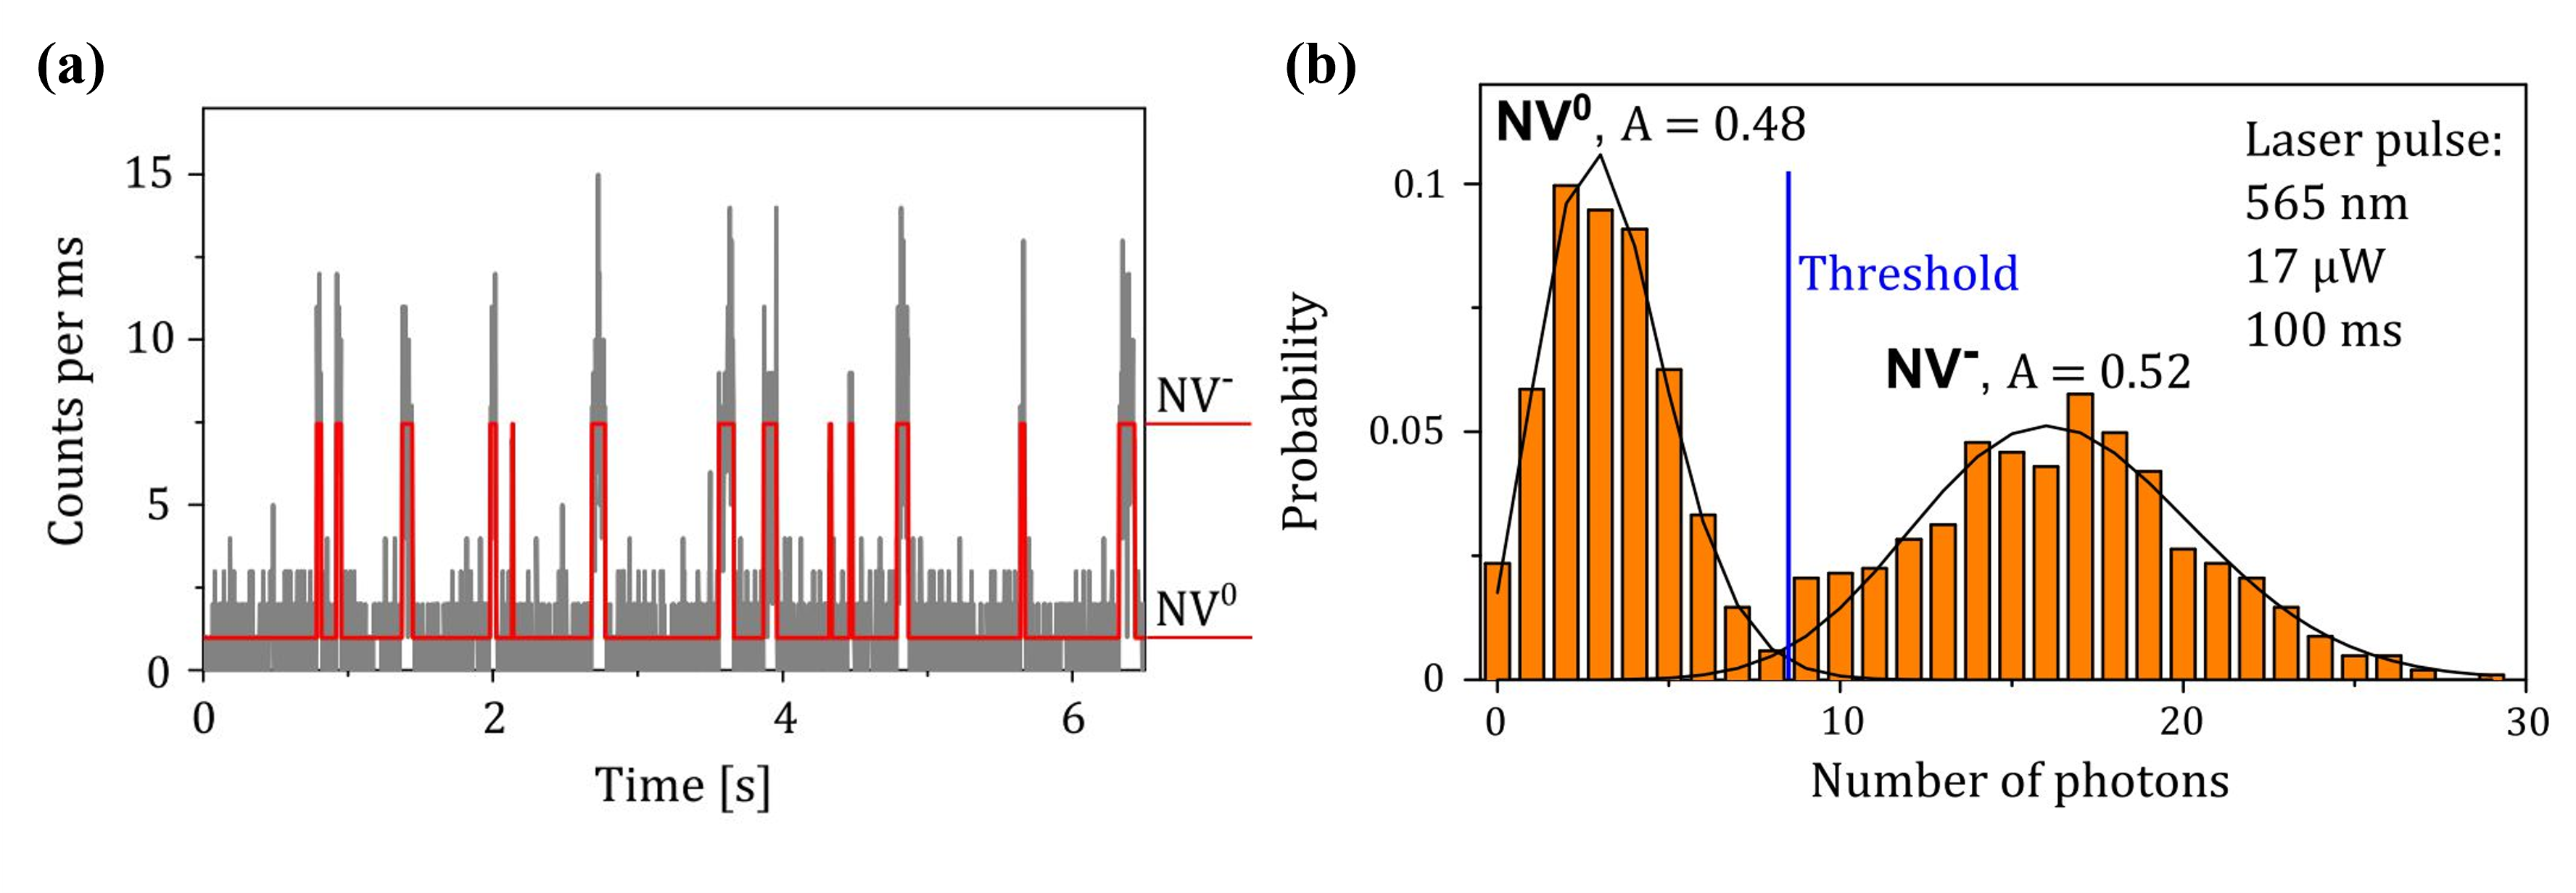
\includegraphics[width=1.0\textwidth]{figures/Chapter 2/n_thresh.png}
  \caption[计数率的统计和$n_{thresh}$的确定]{计数率的统计和$n_{thresh}$的确定,(a)图中展示了APDs计数率随着时间的变化趋势,(b)中的柱状图展示了讲计数率转化为概率密度分布的曲线\cite{aslam2013photo}。}
  \label{fig: n_thresh}
\end{figure}

\subsection{脉冲测量中初始化电荷态和初始化保真度$\mathcal{F}_I$}
当进行脉冲序列测量的时候,电荷态将不会保持一个稳定的状态,而是会随着初始化脉冲和读出脉冲的序列而发生变化。为了初始化电荷态,即将尽可能多的NV$^0$转化到NV$^-$的$m_s=0$态,在594 nm的橙光读出后,会紧跟着一束持续3000 ns的高功率532 nm的绿光脉冲来对NV Center进行初始化。这种方法的原理是基于不同波长的激光会对NV Center的电荷和复合产生比较大的影响。在532 nm的绿光脉冲的作用下,NV$^0$的电子会被激发到更高的能级,从而能和价带中或者电子势阱中的额外电子结合,使得NV Center回到NV$^-$的状态,而NV$^-$在基态三重态$m_s=±1$的电子则会被激发到NV$^-$的激发态,然后通过ISC过程回到NV$^-$的$m_s=0$基态,这样就使得NV Center被初始化。

脉冲测量的主要作用就是确定初始化保真度$\mathcal{F}_I$,而在施加绿光脉冲的过程中,NV$^-$的电离作用主要取决于绿光的功率,也就是说功率过高的绿光会将NV$^-$再次电离,这样就会降低电离的保真度,所以需要对于绿光的功率进行优化,使得初始化保真度$\mathcal{F}_I$达到最大值。$\mathcal{F}_I$可以通过随着时间变化的计数率直方图来计算,通过拟合初始的光子数来得到:
\begin{equation}
  P(n)_{ini}=(1-\mathcal{F}_I)p(n|NV^0)+\mathcal{F}_Ip(n|NV^-)
\end{equation}
其中$p(n|NV^0)$和$p(n|NV^-)$分别是NV$^0$和NV$^-$的概率分布,而$\mathcal{F}_I$则是初始化保真度,即初始化NV$^0$为NV$^-$的概率。在这个模型中,我们假设了在初始化脉冲之后,NV Center的电荷态不会发生改变,即在读出脉冲之前,NV Center的电荷态不会发生改变,这个假设在实验中是成立的,因为初始化脉冲的时间尺度远小于读出脉冲的时间尺度,所以在读出脉冲之前,NV Center的电荷态不会发生改变。

对于初始化保真度的优化同样十分重要,因为初始化脉冲在大部分涉及到NV Center的实验中,通常被用于在测量序列之前让尽可能多的NV Center转化为方便调控和读出的NV$^-$,并且提高NV Center用于量子信息领域时候较为重要的自旋相干时间这一参数\cite{robledo2011spin}。

\end{document}